% arara: lualatex: { interaction: nonstopmode, synctex: no }
% arara: lualatex: { interaction: nonstopmode, synctex: no }
\documentclass[a4paper,12pt,chapterprefix=false,bibliography=totoc,listof=totoc,]{scrreprt}

\usepackage{latex-style}

\lstdefinelanguage{Gherkin}{
	morekeywords = {
		Given,
		When,
		Then,
		And,
		Scenario,
		Feature,
		But,
		Background,
		Scenario Outline,
		Examples
	},
	sensitive=true,
	morecomment=[l]{\#},
	morestring=[b]",
	morestring=[b]',
	keywordstyle=\normalsize\bfseries\color{green},
	basicstyle=\small\ttfamily,
}

\setlength{\parindent}{0pt}

\begin{document}
\begin{flushright}
GameBase
\\
Use-Case Specification: Configure Game Server
% \\
% For <Subsystem or Feature>
\bigbreak
Version 1.1
\end{flushright}

\tableofcontents

\chapter{Use-Case: Configure GameServer}

\section{Brief Description}
The use case describes the configuration of gameservers

\chapter{Flow of Events}
\begin{figure}[H]
	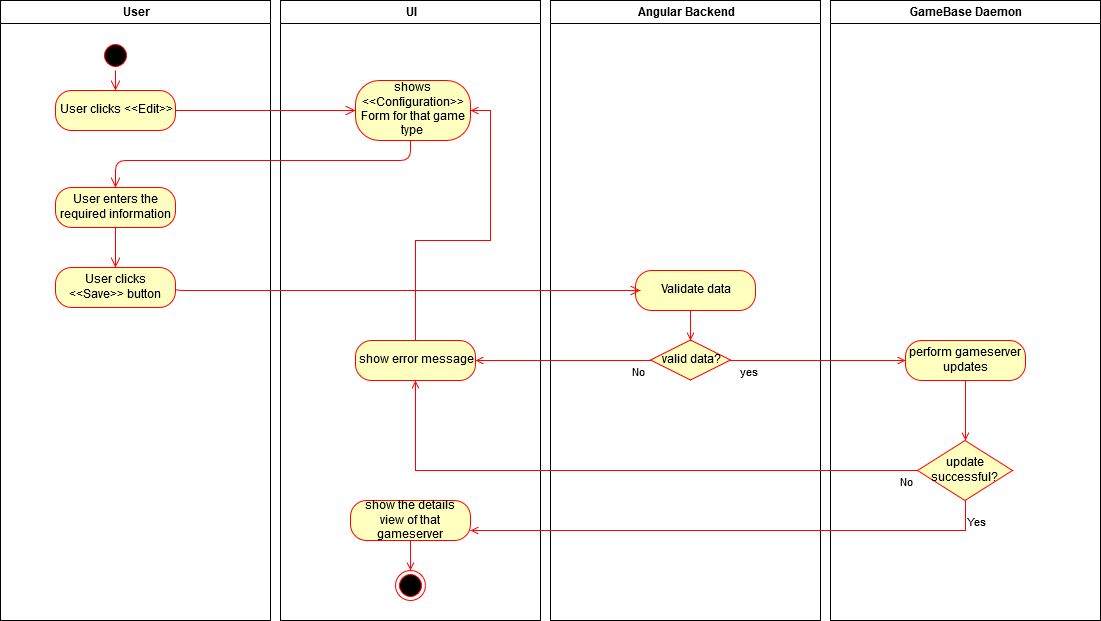
\includegraphics[width=\textwidth]{diagramms/ConfigureGameserverActivityDiagramm.png}
	\caption{Activity Diagramm}
	\label{fig:ad}
\end{figure}

\section{Basic flow}

\begin{itemize}
    \item User is on the Dashboard
    \item User clicks on <<Settings>> cog button
    \item User fills the form with the required information
    \item User clicks on <<Apply>> to save the edits and gets redirected to the Dashboard
    \item or the User clicks on <<Cancel>> to cancel the update operation and gets redirected to the Dashboard
\end{itemize}


\section{.feature File}
\begin{minipage}{\textwidth}
\lstinputlisting[language=Gherkin]{features/configureGameServer.feature}
\end{minipage}

\section{Configuration}
\begin{figure}
    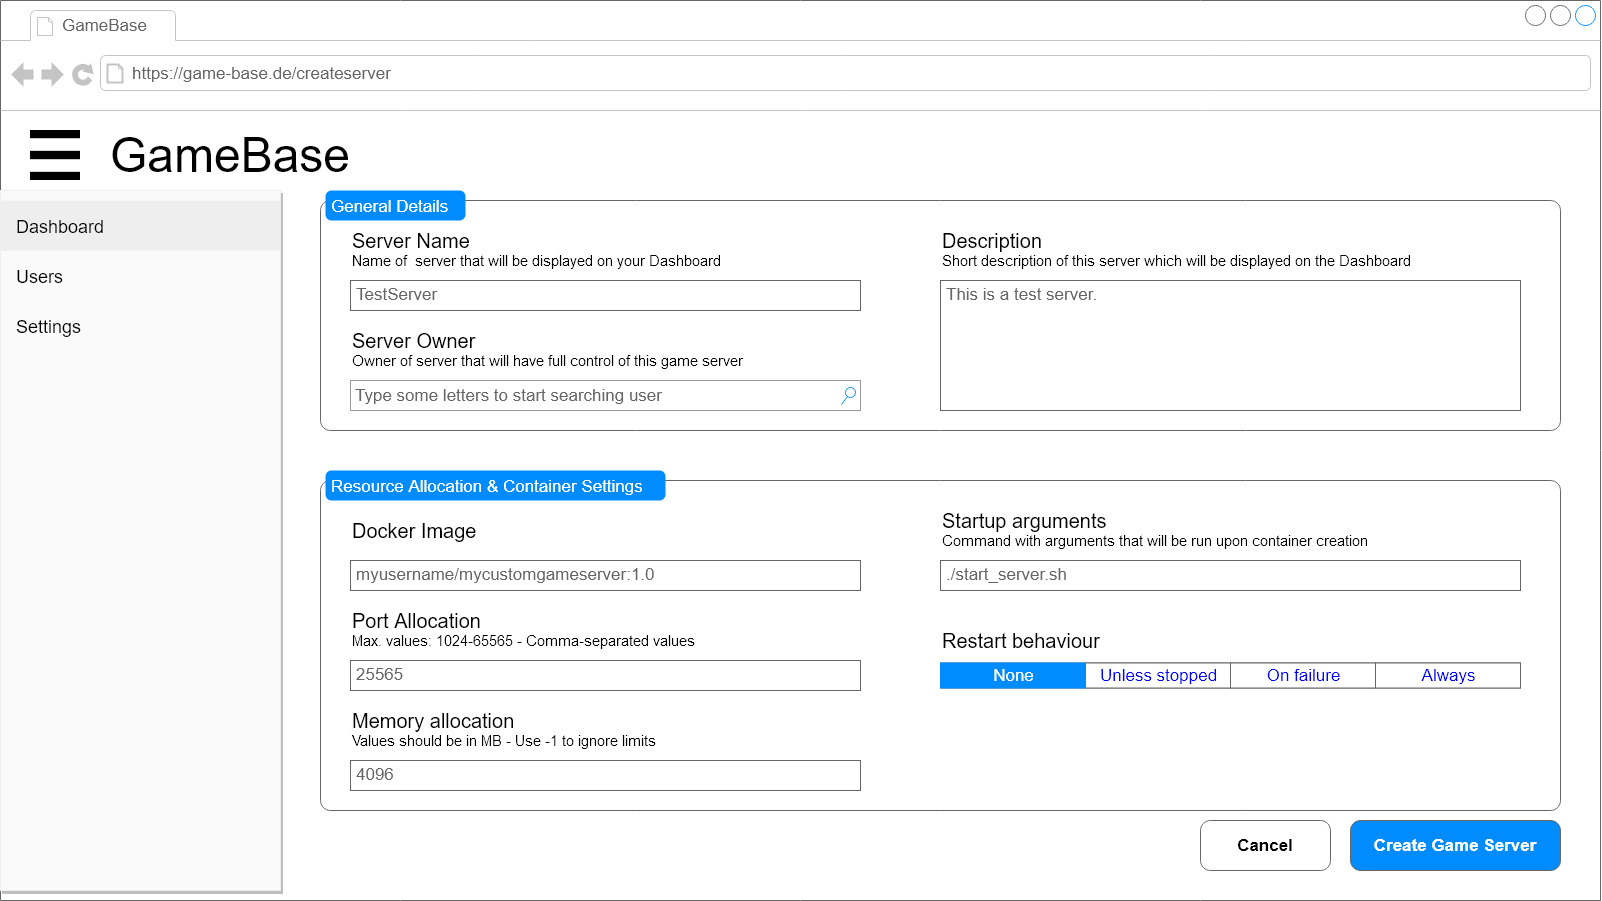
\includegraphics[width=\textwidth]{diagramms/UCConfigureGameServerMockup.jpg}
    \caption{Mockup of the game server configuration page (previously: game server creation wizard)}
    \label{fig:mockup}
\end{figure}
The configuration page is made up of two parts: General Details and Resource Allocation \& Container Settings.

In General Details, the user sets a server name and a short description which will be displayed later on the user's dashboard.

In Resource Allocation \& Container Settings, the user will be asked to select the type (game) of the game server in form of a template with predefined Docker image. In addition, the user can allocate ports and memory for the game server if he chooses to change the standards. This is relevant when e. g. updating the ports used by a gameserver internally. If any additional startup arguments are needed, the user can set them in the box "Startup Arguments". As a last option, the user can choose how the restart behaviour of the container should be.

\chapter{Special Requirements}

\section{Owning an account}
The user has to be a registered user for our system.

\section{Being allowed to configure that gameserver}
The user needs the permissions to update that gameserver.

\chapter{Preconditions}
\section{Must be logged in}
The user must be logged in to edit a server.

\section{Must be owner or permitted to update the server}
The user must own that gameserver or has the permissions to configure the gameserver

\section{User navigated on the gameserver details page}
The user must have navigated on the gameservers details page of the gameserver he wants to edit.

\chapter{Postconditions}

\section{Configure}
After configuring a gameserver the user will be redirected to the gamservers details page.

\end{document}
